\documentclass{article}
\newcommand{\ve}[1]{\mathbf{#1}}
\newcommand{\dd}{\text{d}}
\newcommand{\ba}{\ve{a}}
\newcommand{\bb}{\ve{b}}
\newcommand{\bA}{\ve{A}}
\newcommand{\bu}{\ve{u}}
\newcommand{\bv}{\ve{v}}
\newcommand{\br}{\ve{r}}
\newcommand{\bt}{\ve{t}}
\newcommand{\bn}{\ve{n}}
\newcommand{\bc}{\ve{c}}
\newcommand{\bq}{\ve{q}}
\newcommand{\bff}{\ve{f}}
\newcommand{\bF}{\ve{F}}
\newcommand{\bx}{\ve{x}}
\newcommand{\hx}{\hat{x}}
\newcommand{\hbx}{\hat{\ve{x}}}
\newcommand{\bS}{\ve{S}}
\newcommand{\bU}{\ve{U}}
\newcommand{\bV}{\ve{V}}
\newcommand{\bQ}{\ve{Q}}
\newcommand{\by}{\ve{y}}
\newcommand{\be}{\ve{e}}
\newcommand{\bs}{\ve{s}}
\newcommand{\bp}{\ve{p}}
\newcommand{\bP}{\ve{P}}
\newcommand{\bR}{\ve{R}}
\newcommand{\bM}{\ve{M}}
\newcommand{\bI}{\ve{I}}
\newcommand{\vq}{\vec{q}}
\newcommand{\balpha}{\boldsymbol{\alpha}}
\newcommand{\bkappa}{\boldsymbol{\kappa}}
\newcommand{\bLambda}{\boldsymbol{\Lambda}}
\newcommand{\blambda}{\boldsymbol{\lambda}}
\newcommand{\bmu}{\boldsymbol{\mu}}
\newcommand{\bOmega}{\boldsymbol{\Omega}}
\newcommand{\bomega}{\boldsymbol{\omega}}
\newcommand{\bSigma}{\boldsymbol{\Sigma}}
\newcommand{\bEps}{\boldsymbol{\varepsilon}}
\newcommand{\beps}{\boldsymbol{\varepsilon}}
\newcommand{\heps}{\hat{\varepsilon}}
\newcommand{\bdelta}{\boldsymbol{\delta}}
\newcommand{\vblambda}{\vec{\boldsymbol{\lambda}}}
\newcommand{\vbsigma}{\vec{\boldsymbol{\sigma}}}
\newcommand{\vba}{\vec{\mathbf{s}}}
\newcommand{\vbu}{\vec{\mathbf{u}}}
\newcommand{\vbx}{\vec{\mathbf{x}}}
\newcommand{\vbv}{\vec{\mathbf{v}}}
\newcommand{\vbs}{\vec{\mathbf{s}}}
\newcommand{\vbEps}{\vec{\boldsymbol{\varepsilon}}}
\newcommand{\vbdelta}{\vec{\boldsymbol{\delta}}}
\newcommand\Rey{\mbox{\textit{Re}}}  % Reynolds number
\newcommand\Ca{\mbox{\textit{Ca}}} % Capillary number
\newcommand\ign{\mathrm{ign}}
\newcommand\tign[1]{\tau_{\ign}^{#1}}
\newcommand\btign[1]{\bvec{\tau}_{\ign}^{#1}}
\newcommand{\rmI}{\mathrm{I}}
\newcommand{\pop}[2]{\frac{\partial#1}{\partial#2}}
\newcommand{\poptwo}[3]{\frac{\partial^{2}#1}{\partial#2\partial#3}}
\newcommand\inj{\mathrm{inj}}

\newcommand{\bvec}[1]{\ensuremath{\boldsymbol{#1}}}
\newcommand{\pp}[1]{\ensuremath{\left( #1 \right)}}
\newcommand{\psq}[1]{\ensuremath{{\left[ #1 \right]}}}
\newcommand{\pcr}[1]{\ensuremath{\left\{ #1 \right\}}}

\newcommand{\bnabla}{\mbox{\boldmath{$\nabla$}}}
\newcommand{\Grad}{\bnabla}

\usepackage{stmaryrd}
\usepackage{epsf}
\usepackage{mathtools}
\usepackage{setspace}
\usepackage{enumerate}
\usepackage{fancyhdr}
\usepackage{float}
\usepackage{overcite}
\usepackage{footnote}
\usepackage{scalefnt}
\usepackage{microtype}
\usepackage{xfrac}
\usepackage{sectsty}
\usepackage{rotate}
\usepackage{array}
\usepackage{tabu}
\usepackage{parskip}
\usepackage{amsmath,amsfonts,amssymb,amsthm,mathrsfs,mathtools}
\usepackage{breqn}
\usepackage{graphicx}
\usepackage{xcolor}
\usepackage{multirow}
\usepackage{wrapfig}
\usepackage{enumerate}
\usepackage{colortbl}
\usepackage{hhtensor}
\usepackage{url}
\usepackage{booktabs}
\usepackage{pdflscape}
\usepackage{standalone}
\usepackage{tikz}
\usepackage{pgfplots}
\usepackage{pgfplotstable}
\usepackage{pgfgantt}
%\usepackage{subcaption}
\usepackage[square,sort,comma,numbers]{natbib}
\usepackage[font=footnotesize,format=plain,labelfont=bf]{caption}
\usepackage{subfig}
\usepackage[version=3]{mhchem}
\usepackage[colorinlistoftodos, color=blue!20!white, bordercolor=gray,
textsize=footnotesize,textwidth=1.1in]{todonotes}
\usepackage[left=1in,right=1in,top=1in,bottom=1in]{geometry}
\usepackage{soul}
\setlength\parindent{20pt}
%\usepackage[nooneline,tight,raggedright]{subfigure}

\usepgfplotslibrary{groupplots,external}
\usetikzlibrary{arrows,shapes,spy,matrix,fit,backgrounds,calc,positioning}
\tikzstyle{every picture}+=[remember picture]
\tikzstyle{na} = [baseline=-2ex]

\newcommand\solidrule[1][1cm]{\rule[0.5ex]{#1}{.4pt}}
\newcommand\dashedrule{\mbox{%
    \solidrule[2mm]\hspace{2mm}\solidrule[2mm]\hspace{2mm}\solidrule[2mm]}}

\usepackage{accents}
\newlength{\dhatheight}
\newcommand{\doublehat}[1]{%
    \settoheight{\dhatheight}{\ensuremath{\hat{#1}}}%
    \addtolength{\dhatheight}{-0.35ex}%
    \widehat{\vphantom{\rule{1pt}{\dhatheight}}%
    \smash{\widehat{#1}}}}

%%%%%%%%% SECTIONING STUFF
\makeatletter
\renewcommand{\section}{\@startsection
{section}%
{0}%
{0mm}%
{0.4\baselineskip}%
{0.4\baselineskip}%
{\normalfont\Large\bfseries\color{myBrown}}}%
\makeatother

\makeatletter
\renewcommand{\subsection}{\@startsection
{subsection}%
{1}%
{0mm}%
{0.4\baselineskip}%
{0.4\baselineskip}%
{\normalfont\large\bfseries\color{myBrown}}}%
\makeatother

\makeatletter
\renewcommand{\subsubsection}{\@startsection
{subsubsection}%
{1}%
{0mm}%
{-0.5\baselineskip}%
{0.3\baselineskip}%
{\normalfont\normalsize\bfseries\color{myBrown}}}%
%{\normalfont\normalsize\itshape\centering\color{myBrown}}}%
\makeatother

\renewcommand{\thesection}{\arabic{section}}
\renewcommand{\thesubsection}{\thesection.\arabic{subsection}}

%%%%%%%%% FORMATTING TIDBITS
\definecolor{myTan}{RGB}{205,133,63}
\definecolor{myBrown}{RGB}{155,77,40}
\captionsetup{labelfont={color=myBrown,bf},textfont={color=myTan}}
\newcommand{\HRule}[2]{{\color{myBrown}\rule{#1}{#2}}}
\newcommand{\tPI}[1]{{\color{myBrown}#1}}
\newcommand{\sPI}[1]{\textsc{\color{myBrown}#1}}
\newcommand{\cPI}[1]{\textbf{\color{myBrown}#1}}
\newcommand{\iPI}[1]{\textit{\color{myBrown}#1}}
\newcommand{\lead}[1]{\textit{\color{myBrown}(#1)}}
\newcommand{\tabtit}[1]{\textsc{\color{myBrown}#1}}
\newcommand{\entry}[1]{\mbox{\sffamily\bfseries{#1:}}\hfil}%
\newcommand{\bitem}{\item[{\color{myBrown}$\bullet$}]}
\renewcommand{\footnoterule}{}

\newcommand{\bmath}{\boldsymbol}
\newcommand{\eps}{\varepsilon}
\newcommand{\Dpartial}[2]{\frac{\partial #1}{\partial #2}}
\newcommand{\itemcolor}[1]{% Update list item colour
\renewcommand{\makelabel}[1]{\color{#1}\hfil ##1}}
\newcommand{\fut}{$^*$}
\newcommand{\pas}{$^\dag$}
\def\bm#1{\mbox{\boldmath{$#1$}}}
\newif\ifclean
\cleantrue
\newcommand{\Jcal}{\mathcal{J}}
\newcommand{\Lcal}{\mathcal{L}}

%% \makeatletter
%% \newcounter{reaction}
%%% >> for article <<
%% \renewcommand\thereaction{C\,\arabic{reaction}}
%%% << for article <<
%%% >> for report and book >>
%% \renewcommand\thereaction{R\,\arabic{reaction}}
%% \@addtoreset{reaction}{chapter}
%%% << for report and book <<
%% \newcommand\reactiontag%
%%   {\refstepcounter{reaction}\tag{\thereaction}}
%% \newcommand\reaction@[2][]%
%%   {\begin{equation}\ce{#2}%
%%   \ifx\@empty#1\@empty\else\label{#1}\fi%
%%   \reactiontag\end{equation}}
%% \newcommand\reaction@nonumber[1]%
%%   {\begin{equation*}\ce{#1}\end{equation*}}
%% \newcommand\reaction%
%%   {\@ifstar{\reaction@nonumber}{\reaction@}}
%% \makeatother

\definecolor{RYB1}{RGB}{207, 37, 37}
\definecolor{RYB2}{RGB}{37, 91, 207}
\definecolor{RYB3}{RGB}{37, 207, 91}
\definecolor{RYB4}{RGB}{163,26,145}
\definecolor{RYB5}{RGB}{253, 180, 98}
\definecolor{RYB6}{RGB}{179, 222, 105}
\definecolor{RYB7}{RGB}{128, 177, 211}

\pgfplotscreateplotcyclelist{newcolors}{
{RYB1,every mark/.append style={fill=RYB1,mark size={2.5}},mark=*},
{RYB2,every mark/.append style={fill=RYB2},mark=square*},
{RYB3,every mark/.append style={fill=RYB3,mark size={3}},mark=triangle*},
{RYB4,every mark/.append style={fill=RYB4,mark size={3}},mark=diamond*},
{RYB5,every mark/.append style={fill=RYB5,mark size={3}},mark=pentagon*},
{RYB6,every mark/.append style={fill=RYB6,mark size={4}},mark=10-pointed star},
{RYB7,every mark/.append style={fill=RYB7},mark=*},
}

\pgfplotsset{compat=1.14}
\pagenumbering{arabic}

\DeclareMathOperator*{\argmin}{arg\,min}

\renewcommand{\eqref}[1]{(\ref{eq:#1})}
\newcommand{\eqrefs}[2]{(\ref{eq:#1})-(\ref{eq:#2})}

\newcommand{\todoECG}[1]{\todo[linecolor=blue,backgroundcolor=blue!25,bordercolor=blue,inline]{\textbf{ECG}:\, $(\uparrow)$\, #1}}

%\usepackage{xcolor}
\usepackage{tikz}
\usepackage{stackrel}
\usepackage{bm,bbm}% bold math
\usepackage[version=3]{mhchem}

\usepackage{multirow}
\usepackage{setspace}
\usepackage{yfonts}
\usepackage{mathrsfs}
\usepackage{tcolorbox}
\usepackage{colortbl}
\usepackage{commath}
\usepackage{multicol}
\usepackage{lmodern}
\usepackage{makecell}
\usepackage{rotating}

% Support for Pandoc-beamer
\usepackage[T1]{fontenc}
\usepackage{booktabs}
\usepackage{longtable}
\usepackage{fancyvrb}
\providecommand{\tightlist}{%
  \setlength{\itemsep}{0pt}\setlength{\parskip}{0pt}}

\usepackage[retainorgcmds]{IEEEtrantools}
\usepackage{siunitx}     
\sisetup{detect-display-math=true,detect-weight=true,detect-family=true}

\usepackage{tcolorbox,xcolor,framed}
\DefineVerbatimEnvironment{Highlighting}{Verbatim}{fontsize=\footnotesize,commandchars=\\\{\}}
\definecolor{shadecolor}{rgb}{0.9,0.9,0.9}
\newenvironment{Shaded}{\snugshade}{\endsnugshade}
\newcommand{\KeywordTok}[1]{\textcolor[rgb]{0.13,0.29,0.53}{\textbf{#1}}}
\newcommand{\DataTypeTok}[1]{\textcolor[rgb]{0.13,0.29,0.53}{#1}}
\newcommand{\NormalTok}[1]{#1}
\newcommand{\DecValTok}[1]{\textcolor[rgb]{0.00,0.00,0.81}{#1}}
\newcommand{\CommentTok}[1]{\textcolor[rgb]{0.56,0.35,0.01}{\textit{{#1}}}}
\newcommand{\PreprocessorTok}[1]{\textcolor[rgb]{0.56,0.35,0.01}{\textit{{#1}}}}
\newcommand{\ControlFlowTok}[1]{\textcolor[rgb]{0.13,0.29,0.53}{\textbf{{#1}}}}


\usepackage[colorinlistoftodos, color=blue!20!white, bordercolor=gray,
textsize=tiny]{todonotes}

\setbeamercolor{structure}{fg=myOrange}
\setbeamercolor{normal text}{fg=myBlue}

\makeatletter
\newcommand*{\overlaynumber}{\number\beamer@slideinframe}
\makeatother

\usepackage{pgf}
\usetikzlibrary{arrows,shapes,shapes.arrows,positioning,calc,decorations.text}

\usepackage{standalone}

\usetheme{default}

\usepackage{multimedia}
\usepackage{media9}

\usepackage{graphicx}
\usepackage{animate}
%\usepackage{minted}


\definecolor{RED}{RGB}{255,0,0}  %%% 
\definecolor{myBlue}{RGB}{19,41,75}  %%% BLUE
\definecolor{myBlueLink}{RGB}{70,70,200}  %%% ILLINOIS BLUE
\definecolor{myOrange}{RGB}{232,74,39}   %%% ILLINOIS ORANGE
\definecolor{IllinoisOrange}{RGB}{232,74,39}  %%% ILLINOIS ORANGE
\definecolor{IllinoisBlue}{RGB}{19,41,75}   %%% ILLINOIS BLUE
\definecolor{mainTextColor}{RGB}{19,41,75}  %%% ILLINOIS BLUE
\definecolor{myLightGray}{rgb}{0.95,0.95,0.95} 
\definecolor{myGold}{rgb}{1.0,.75,0.0} 


%%% Modify the footline to only have the page numbering in the center, nothing else
\makeatletter
\setbeamertemplate{footline}
{
 \leavevmode%
 \hbox{\begin{beamercolorbox}[wd=\paperwidth,ht=2.25ex,dp=1ex,center]{}%
   \usebeamerfont{author in head/foot}\insertframenumber{}%
 \end{beamercolorbox}}
 \vskip0pt%
}

%%% Modify the headline to be null
\setbeamertemplate{headline}{}

%%% Set frame title to be transparent with black text
\setbeamercolor{frametitle}{bg=}
\setbeamercolor{frametitle}{fg=myOrange}


%%% Set frame title to properly center the text
\setbeamertemplate{frametitle}
{
  \leavevmode%
  \hbox{%
  \begin{beamercolorbox}[wd=\paperwidth,ht=2.5ex,dp=0ex]{frametitle}%
    \raggedright
    \bfseries
    \hspace*{0.3em}%
    \usebeamerfont{frametitle}\insertframetitle
  \end{beamercolorbox}}
  \vspace*{-2.75ex}
}


\makeatother

\setbeamersize{text margin left=0.15in,text margin right=0.15in}

%%% turn off navigation line (uncomment to reinstate)
\setbeamertemplate{navigation symbols}{}

%%% turn off the balls for enumerate
\setbeamertemplate{enumerate items}[default]
% \setbeamertemplate{itemize items}[default]

\setbeamertemplate{itemize subitem}{$\bullet$}
\setbeamertemplate{itemize subsubitem}{$*$}


%%% Set the background image
\usebackgroundtemplate%
{%
    
\includegraphics[width=\paperwidth]{ceesd-slide-background.pdf}%
}



\def\Put(#1,#2)#3{\leavevmode\makebox(0,0){\put(#1,#2){#3}}}
\newcommand{\prj}[2]{{\color{gray} #1 [#2]}}
\newcommand{\noprj}[2]{}
\newcommand{\talkref}[2]{{\color{gray} #1 [#2]}}
\newcommand{\makered}[1]{{\color{red} #1}}
\newcommand{\makeblue}[1]{{\color{blue} #1}}
\newcommand{\makegreen}[1]{{\color{green} #1}}
\newcommand{\maketeal}[1]{{\color{teal} #1}}
\newcommand{\makeorange}[1]{{\color{orange} #1}}
\newcommand{\makeRed}[1]{{\color{red} #1}}
\newcommand{\makeBlue}[1]{{\color{blue} #1}}
\newcommand{\makeCyan}[1]{{\color{cyan} #1}}
\newcommand{\makeOrange}[1]{{\color{orange} #1}}
\newcommand{\makeGreen}[1]{{\color{ForestGreen} #1}}
\newcommand{\makeGold}[1]{{\color{myGold} #1}}

\newcommand{\clink}{{\tiny({\color{blue} link})}}


\newcommand{\myoul}[1]{\color{myBlue}\underline{\smash{\color{myOrange} #1}}\color{myOrange}}
\newcommand{\ccdot}{\color{myBlue}$\circ$\color{myOrange}\;}
\newcommand{\cc}[1]{\color{myBlue}#1\color{myOrange}{}}

\newcommand{\HRule}[2]{{\color{myBlue}\rule{#1}{#2}}}
\newcommand{\dRightarrow}{{\color{myOrange}\Rightarrow}}
\newcommand{\dLeftarrow}{{\color{myBlue}\Leftarrow}}
\newcommand{\tb}[1]{{\color{blue}(#1)}}
\newcommand{\tr}[1]{{\color{blue}({\color{red}#1})}}
\newcommand{\tor}[1]{{\color{blue}({\color{blue}#1})}}
\newcommand{\lead}[1]{\textit{\color{myBlue}(#1)}}
\newcommand{\bmath}{\boldsymbol}
\newcommand{\eps}{\varepsilon}
\newcommand{\vp}{\vec{p}}
\newcommand{\rPI}[1]{{\color{myOrange}#1}}
\newcommand{\tPI}[1]{\texttt{\color{myOrange}#1}}
\newcommand{\ttPI}[1]{\texttt{\color{myOrange}#1}}
\newcommand{\cPI}[1]{\textbf{\color{myOrange}#1}}
\newcommand{\iPI}[1]{\textit{\color{myOrange}#1}}
\newcommand{\sPI}[1]{\textsc{\color{myOrange}#1}}
\newcommand{\scPI}[1]{\textsc{\color{myOrange}#1}}
\newcommand{\tabtit}[1]{\textsc{\color{myOrange}#1}}
\newcommand{\Dpartial}[2]{\frac{\partial #1}{\partial #2}}
\newcommand{\bx}{\mathbf{x}}
\newcommand{\bU}{\mathbf{U}}
\newcommand{\obsigma}{{\bar \sigma}}
\newcommand{\vsigma}{\vec{\sigma}}
\newcommand{\II}{{I\!I}}
\newcommand{\memph}[1]{{\color{red} #1}}
\newcommand{\eg}{\emph{e.g.}}
\newcommand{\mat}[1]{\ensuremath{\mathsf{#1}}}
\newcommand{\bvec}[1]{\ensuremath{\boldsymbol{#1}}}



\newcommand{\sectionWithFrame}[1]{%
  \section{#1}
  \begin{frame}
    \centerline{\LARGE \insertsection}
  \end{frame}}
\newcommand{\sectionAndsubWithFrame}[2]{%
  \section{#1}
  \begin{frame}
    \centerline{\LARGE \insertsection}
    \bigskip
    \centerline{\large #2}
  \end{frame}}

\newcommand{\cM}{\mathcal{M}}

\newcommand{\bn}{\mathbf{n}}

\newcommand{\bbC}{\mathbb{C}}
\newcommand{\vbbm}{{\vec{m}}}
\newcommand{\bbM}{\mathbb{M}}
\newcommand{\bbH}{\mathbb{H}}
\newcommand{\bbG}{\mathbb{G}}
\newcommand{\bbV}{\mathbb{V}}

\newcommand{\vD}{{\vec D}}
\newcommand{\vhD}{{\hat{D}}}
\newcommand{\vg}{{\vec g}}
\newcommand{\vphi}{{\vec\phi}}
\newcommand{\vOmega}{{\vec\Omega}}

\newcommand{\vF}{{\vec{F}}}
\newcommand{\vf}{{\vec{f}}}
\newcommand{\vb}{{\vec{b}}}
\newcommand{\vq}{{\vec{q}}}
\newcommand{\vqs}{{\vec{q}^{\,\color{red}*}}}

\newcommand{\cJ}{\mathcal{J}}
\newcommand{\cK}{\mathcal{K}}
\newcommand{\cG}{\mathcal{G}}
\newcommand{\cI}{\mathcal{I}}
\newcommand{\cP}{\mathcal{P}}
\newcommand{\cN}{\mathcal{N}}
\newcommand{\cC}{\mathcal{C}}
\newcommand{\cO}{\mathcal{O}}
\newcommand{\cS}{\mathcal{S}}
\newcommand{\cQ}{\mathcal{Q}}

\newcommand{\rstar}{{\color{red}*}}
\newcommand{\rchk}{{\color{red} \checkmark}}
\newcommand{\gchk}{{\color{green} \checkmark}}
\newcommand{\rbul}{{\color{red} $\bullet$}}
\newcommand{\pbul}{{\color{myOrange} $\bullet$}}
\newcommand{\bbul}{{\color{blue} $\bullet$}}
\newcommand{\gbul}{{\color{green} $\bullet$}}
\newcommand{\po}{{\color{myOrange} $\circ$}}
\newcommand{\ro}{{\color{red} $\circ$}}
\newcommand{\bd}{{\color{blue} $\bullet$}}

\newcommand{\rhoi}[1][i]{\rho_{#1}}
\newcommand{\dt}[1][t]{\partial_{#1}}
\newcommand{\dx}[1][{\textrm{\bf x}}]{\boldsymbol \partial_{#1}}
\newcommand{\Vi}[1][i]{\mathcal{V}_{#1}}
\newcommand{\Mi}[1][\textswab{i}]{\mathcal{M}_{#1}}
\newcommand{\omegai}[1][i]{\dot{\omega}_{#1}}
\newcommand{\grav}{{\bf g}}
\newcommand{\Etot}{\mathcal{E}}

\newcommand{\mBG}{m_{\text{\tiny BG}}}
\newcommand{\nBG}{n_{\text{\tiny BG}}}
\newcommand{\nIp}{n_{\text{\tiny $I^+$}}}
\newcommand{\nIm}{n_{\text{\tiny $I^-$}}}


\newcommand{\bI}{{\mathbf{I}}}
\newcommand{\bq}{{\mathbf{q}}}
\newcommand{\btau}{{\boldsymbol{\tau}}}

\newcommand{\bv}{{\bar{v}}}
\newcommand{\bepsilon}{{\bar{\epsilon}}}

\newcommand{\ST}{{S_{\text{\tiny T}}}}

\newcommand{\vu}{\vec{u}}
\newcommand{\vQ}{\vec{Q}}
\newcommand{\veta}{\vec{\eta}}


  \newcommand{\Grad}{\bnabla}
  \newcommand{\Div}{\bnabla\vdot}
  \newcommand{\Curl}{\bnabla\vprod}
  \newcommand{\hGrad}{\bnabla^{}_{\!\!\mathrm{h}}}
  \newcommand{\hDiv}{\bnabla^{}_{\!\!\mathrm{h}}\!\vdot}
  \newcommand{\pGrad}{\bnabla^{}_{\!\!\!\perp}}
  \newcommand{\pDiv}{\bnabla^{}_{\!\!\!\perp}\!\vdot}
\newcommand{\pop}[2]{\frac{\partial #1}{\partial #2}}
\newcommand{\pp}[1]{\ensuremath{\left[ #1 \right]}}
\newcommand{\psq}[1]{\ensuremath{{\left[ #1 \right]}}}

% Grad, div, curl, etc.
\newcommand{\vdot}{\mathop{\mbox{\boldmath{$\cdot$}}}}
\newcommand{\vddot}{\mathop{\mbox{\textbf{:}}}}
\newcommand{\bnabla}{\mbox{\boldmath{$\nabla$}}}
\newcommand{\Lapl}{\nabla^2}
\newcommand{\hLapl}{\nabla^2_{\!\mathrm{h}}}
\newcommand{\pLapl}{\nabla^2_{\!\!\!\perp}}

\newcommand{\kION}{k_{\text{\tiny ION}}}
\newcommand{\kDET}{k_{\text{\tiny DET}}}
\newcommand{\kDR}{k_{\text{\tiny DR}}}
\newcommand{\kDA}{k_{\text{\tiny DA}}}
\newcommand{\kII}{k_{\text{\tiny $II$}}}


\def\colorize<#1>{%
\temporal<#1>{}{\color{red}}{}
}

\newcommand{\paper}[1]{ {\tiny #1\par} }
\newcommand{\TODO}[1]{{\color{red} \tiny TODO: #1}}
\newcommand{\CHK}{{\color{red} ???}}
\newcommand{\CHKWDG}{{\color{red} ???WDG???}}
\newcommand{\progname}[1]{\textit{#1}}
\newcommand{\PlasComCM}{\progname{PlasComCM}}
\newcommand{\PlasComCMtwo}{\progname{PlasCom2}}
\newcommand{\plascomtwo}{\progname{PlasCom2}}
\newcommand{\plusplus}[1]{#1{}\texttt{++}}
\newcommand{\ceesdcode}{\textit{MIRGE-Com}}
\newcommand{\ceesdMIRGE}{\textit{MIRGE}}
\newcommand{\ceesdbasiccode}{\textit{M-Com}}
\newcommand{\ABaTe}{\textit{A\!Ba\!Te}}
\newcommand{\codelet}[1]{\progname{Codelet-#1}}
\newcommand{\goldenCopy}{\rPI{golden copy}}
\newcommand{\GoldenCopy}{\rPI{Golden copy}}
\newcommand{\code}[1]{\texttt{#1}}
\newcommand{\PCtwo}{\progname{PlasCom2}}
\newcommand{\CSTUF}{\progname{CSTUF}}

\newcommand{\xnew}{$^{\text{\tiny \makered{new}}}$}
\newcommand{\xremind}{$^{\text{\tiny \makeblue{reminder}}}$}
\newcommand{\Q}[1]{{\medskip\small\noindent\color{blue}\itshape
    $\bullet$ #1\par}}
\newcommand{\Qi}[1]{\begin{center}\begin{minipage}{0.9\textwidth}\footnotesize\noindent\color{blue}\itshape
    $\circ$ #1\par\end{minipage}\end{center}\vspace*{-0.2in}}

\newcommand{\insertmovie}[3]{\ifmovies{
\movie[autostart,loop]
{\includegraphics[width=#1\textwidth]{Movies/#2}}
{Movies/#3}
}
\else{
\includegraphics[width=#1\textwidth]{Movies/#2}
}
\fi
}

\usefonttheme[onlymath]{serif}

\definecolor{ForestGreen}{rgb}{0.0, 0.2, 0.13}
\definecolor{darkpastelgreen}{rgb}{0.01, 0.75, 0.24}
\definecolor{antiquewhite}{rgb}{0.98, 0.92, 0.84}

\newcommand{\planA}{$\mathbb{A}$}
\newcommand{\planAA}{$\mathcal{A}'$}
\newcommand{\planB}{B}

\newcommand{\MUST}{{\footnotesize\color{red} \textbf{MUST}}}
\newcommand{\WISH}{{\footnotesize\color{orange} \textbf{WISH}}}
\newcommand{\DEFER}{{\footnotesize\color{yellow} \textbf{DEFER}}}
\newcommand{\WDEFER}{{\footnotesize\color{lightgray} \textbf{DEFER}}}
\newcommand{\RETURN}{{\footnotesize\color{blue} \textbf{RETURN}}}
\newcommand{\DONE}{{\footnotesize\color{ForestGreen} \textbf{COMPLETED}}}
\newcommand{\PLAN}{{\footnotesize\color{green} \textbf{PLANNED}}}
\newcommand{\CURRENT}{{\footnotesize\color{cyan} \textbf{NOW}}}

\newcommand{\SNL}{{\footnotesize $\;\rightarrow$ SNL}}
\newcommand{\LLNL}{{\footnotesize $\;\rightarrow$ LLNL}}
\newcommand{\LANL}{{\footnotesize $\;\rightarrow$ LANL}}


\newcommand{\aMUST}{\tiny\raisebox{1.5pt}{\color{red} (\textbf{M})}}
\newcommand{\aWISH}{\raisebox{1.5pt}{\tiny\color{orange} (\textbf{W})}}
\newcommand{\aDEFER}{\raisebox{1.5pt}{\tiny\color{yellow} (\textbf{D})}}
\newcommand{\aRETURN}{\raisebox{1.5pt}{\tiny\color{blue} (\textbf{R})}}
\newcommand{\aDONE}{\raisebox{1.5pt}{\tiny\color{ForestGreen} (\textbf{C})}}
\newcommand{\aPLAN}{\raisebox{1.5pt}{\tiny\color{green} (\textbf{P})}}
\newcommand{\aCURRENT}{\raisebox{1.5pt}{\tiny\color{cyan} (\textbf{N})}}

\newcommand{\Resp}{\cPI{Planned Response}}
\newcommand{\Recm}{\cPI{Recommendation}}

\newcommand{\gdotfill}{{\color{gray}\dotfill}}

\newcommand{\later}[1]{\centerline{\color{myOrange} \ldots #1}}
\newcommand{\recbox}[1]{
\fcolorbox{myBlue}{antiquewhite}{
\begin{minipage}{0.97\textwidth}
\noindent
\Recm:
{#1}
\end{minipage}}
}
\newcommand{\recb}[1]{\fcolorbox{myBlue}{antiquewhite}{\Recm: #1}}

\newcommand{\recboxnt}[1]{
\fcolorbox{myBlue}{antiquewhite}{
\begin{minipage}{0.97\textwidth}
{#1}
\end{minipage}}
}

\arrayrulecolor{myOrange}

\usepackage{pgfplots}
\usepackage{pgfplotstable}

\definecolor{RYB1}{RGB}{207, 37, 37}
\definecolor{RYB2}{RGB}{37, 91, 207}
\definecolor{RYB3}{RGB}{37, 207, 91}
\definecolor{RYB4}{RGB}{163,26,145}
\definecolor{RYB5}{RGB}{253, 180, 98}
\definecolor{RYB6}{RGB}{179, 222, 105}
\definecolor{RYB7}{RGB}{128, 177, 211}

\pgfplotscreateplotcyclelist{newcolors}{
{RYB1,every mark/.append style={fill=RYB1,mark size={2.5}},mark=*},
{RYB2,every mark/.append style={fill=RYB2},mark=square*},
{RYB3,every mark/.append style={fill=RYB3,mark size={3}},mark=triangle*},
{RYB4,every mark/.append style={fill=RYB4,mark size={4}},mark=x},
{RYB5,every mark/.append style={fill=RYB5,mark size={3}},mark=oplus},
%{RYB6,every mark/.append style={fill=RYB6,mark size={4}},mark=10-pointed star},
{RYB7,every mark/.append style={fill=RYB7},mark=*},
}
\pgfplotsset{
  %  every axis/.append style={
 %       scale only axis,
 %      width=0.5\textwidth,
%    },
    standard/.style={
    thick,
    compat=1.8,
            scale only axis,
        width=0.45\textwidth,
  %      axis x line=middle,
%        axis y line=middle,
        enlarge x limits=0.05,
        enlarge y limits=0.05,
  %      every axis x label/.style={at={(current axis.right of origin)},anchor=north west},
  %      every axis y label/.style={at={(current axis.above origin)},anchor=north east},
        max space between ticks=40,
 %       tick label style={font=\Large},
%label style={font=\Large},
%legend style={font=\Large},
cycle list name=newcolors
%    cycle list={RYB1\\RYB2\\RYB3\\RYB4\\RYB5}
    }
}


\begin{document}
  
\section{Problem Target}\label{sec:experiment}
  
  Description of the problem we are trying to solve (experiment)
  
\section{Governing Equations}\label{subsec:gov_equations}

We solve the compressible reactive flow equations
\begin{equation}\label{eq:gov_eqns}
  \pop{\bvec{Q}}{t} + \pop{\bvec{F}_{i}^{I}}{x_{i}} - \pop{\bvec{F}_{i}^{V}}{x_{i}} - \bvec{S} = \bvec{0},
\end{equation}
where $\bvec{Q} = [ \rho,\, \rho u_{i},\, \rho E,\, \rho Y_{k} ]$ is the vector of conserved variables, with $\rho$ the density, $\rho u_{i}$ the momentum in the $i^{\mathrm{th}}$ direction, $\rho E$ the total energy density
\begin{equation}
  \rho E = \frac{1}\rho u_{i}u_{i} + \sum_{i = 1}^{N}\rho Y_{k} e_{k},
\end{equation}
where $e_{k}$ and $\rho Y_{k}$ are the internal energy and density of the $k^{\mathrm{th}}$ species for $k = 1,\dots,N-1$. The $N^{\mathrm{th}}$ species is $\ce{N2}$ and is treated as abundant, so its density is computed from
\begin{equation}\label{eq:mass_abund}
  \rho Y_{N} = \rho - \sum_{k = 1}^{N-1}\rho Y_{k}.
\end{equation}
The inviscid $\bvec{F}_{i}^{I}$ and viscous $\bvec{F}_{i}^{V}$ fluxes, and source terms $\bvec{S}$ are
\begin{equation}\label{eq:fluxes}
  \bvec{F}_{i}^{I} = \begin{bmatrix}
    \rho u_{i} \\
    \rho u_{1}u_{i} + p \delta_{i1} \\
    \rho u_{2}u_{i} + p \delta_{i2} \\
    \rho u_{3}u_{i} + p \delta_{i3} \\
    u_{i}( \rho E + p ) \\
    \rho Y_{k} u_{i}
  \end{bmatrix},\quad
  \bvec{F}_{i}^{V} = \begin{bmatrix}
    0 \\
    \tau_{1i} \\
    \tau_{2i} \\
    \tau_{3i} \\
    u_{j}\tau_{ij} - q_{i} \\
    \varphi_{ki}
  \end{bmatrix},\quad
  \bvec{S} = \begin{bmatrix}
    0 \\
    0 \\
    0 \\
    0 \\
    0 \\
    W_{k}\dot{\omega}_{k}
  \end{bmatrix},
\end{equation}
where $p$ is the pressure, $\delta_{ij}$ is the Kronecker delta, $\tau_{ij}$ the viscous stress tensor, $q_{i}$ the heat flux, $\varphi_{k,i}$ the diffusion flux of species $k$, $W_{k}$ its molecular weight and $\dot{\omega}_{k}$ its net chemical production rate. \\

Models for the viscous stress tensor $\tau_{ij}$, heat flux $q_{i}$, diffusion fluxes $\varphi_{ki}$, and net production rates $\dot{\omega}_{i}$ must be specified to close~\eqref{gov_eqns}. The viscous stress tensor is that of a Newtonian fluid,
\begin{equation}\label{eq:vstress_tens}
  \tau_{ij} = 2\mu\psq{S_{ij} - \frac{1}{3}\pop{u_{m}}{x_{m}}},
\end{equation}
where $\mu$ is the dynamic viscosity and
\begin{equation}\label{eq:strain_rate}
  S_{ij} = \frac{1}{2}\pp{ \pop{u_{i}}{x_{j}} + \pop{u_{j}}{x_{i}} }.
\end{equation}
is the strain-rate tensor. The heat flux is
\begin{equation}\label{eq:heat_flux}
  q_{i} = -\pop{(\lambda\, T)}{x_{i}} + h_{k} \varphi_{ki},
\end{equation}
where $\lambda$ is the thermal conductivity and $h_{k}$ is enthalpy of species $k$. The diffusion fluxes are
\begin{align}\label{eq:diff_vel}
  \varphi_{ki} &= \varphi_{k,i}^{\ast} + \varphi_{ki}^{c}, \\
  \varphi_{ki}^{\ast} &= -\rho D_{k,m}\frac{W_{k}}{W}\pop{X_{k}}{x_{i}}, \\
  \varphi_{ki}^{c} &= -Y_{k}\sum_{n = 1}^{N}\varphi_{ni}^{\ast},
\end{align}
where $\varphi_{k,i}^{\ast}$ is its mixture-average approximation, $\varphi_{ki}^{c}$ a correction flux to ensure mass conservation, $D_{k,m}$ the mixture-averaged diffusivity of species $k$, $X_{k} = W_{(k)}Y_{k}/W$ its mole fraction (where the parenthesis precludes summation over repeated indices), and $W$ the mean molecular weight. The net production rates are given by
\begin{equation}\label{eq:omega}
  \dot{\omega}_{k} = \nu_{kr}R_{r}
\end{equation}
where $\nu_{kr}$ is the net stoichiometric coefficient of species $k$ in reaction $r$, and $R_{r}$ is the rate of progress of reaction $r$, the specific form of which is readily available~\cite{ref:Glassman2014,ref:Williams2018}. \\

\subsection{Boundary Conditions}\label{subsec:boundary_conditions}

Navier--Stokes characteristic boundary conditions~\cite{ref:PoinsotLele1992} are enforced at the combustor inlet and (supersonic inflow and non-reflective outflow), injector inlet (supersonic inflow), and the walls (no-slip). Walls are taken to be impermeable~\cite{ref:YooIm2007,ref:Kolla2012},
\begin{equation}
  n_{i}\varphi_{ki} = 0,
\end{equation}
for $i = 1,\dots,N$, where $n_{i}$ is the wall-normal vector. \\
  
To absorb outgoing disturbances and minimize reflections from computational boundaries, absorbing buffer zones are used near the boundaries~\cite{ref:Freund1997,ref:Colonius2004}. In these zones, a source term
\begin{equation}
  S_{b} = -\Upsilon(\bvec{x})\pp{\frac{ \bvec{Q} - \bvec{Q}_{\mathrm{ref}} }{ \tau_{b} }}
\end{equation}
is added to~\eqref{gov_eqns} to penalize deviations from a prescribed reference state at the boundary $\bvec{Q}_{\mathrm{ref}}$, where $\Upsilon$ is the buffer's support, $\tau_{b}$ is the time scale over which the penalty acts. Here, we use
\begin{align}
  \tau_{b} &= \frac{ | \bvec{x}_{b} - \bvec{x}_{0} | }{ 1.25\,c_{\mathrm{ref}} }, \\
  \Upsilon(\bvec{x}) &= \pp{ \frac{ | \bvec{x} - \bvec{x}_{0} | }{ | \bvec{x}_{b} - \bvec{x}_{0} | } }^{2},
\end{align}
where $\bvec{x}_{b}$ and $\bvec{x}_{0}$ denotes the boundary and the end of the buffer zone, and $c_{\mathrm{ref}}$ is the reference speed of sound at the boundary.

\subsection{Equation of State}\label{subsec:eos}

\section{Numerical Model}\label{sec:model}

DG stuff goes here

\section{Numerical Setup}\label{sec:numsetup}


mesh stuff
initialization stuff

\section{Example Results}\label{sec:results}


\newpage
\bibliographystyle{unsrtnat}
\bibliography{ref}





%%======================================================================
%\begin{frame}\frametitle{Overview}
%
%\begin{itemize}
%
%\item ACT-II facility, experimental basis
%\item Numerical Model
%\item Simulation Initialization
%\item Sample results
%
%\end{itemize}
%
%\end{frame}
%
%%======================================================================
%  
%  \begin{frame}\frametitle{ACT-II Experimental Facility}
%  
%  \vspace*{0.15in}
%  \begin{itemize}
%  \setlength{\itemsep}{0.15in}
%  \item \cPI{ACT-II}:  on-campus AFOSR-funded supersonic combustion facility
%  \item Arcjet driven: low cost ($\lesssim$ \$10), low turnaround
%    time ($\lesssim$ 10\,min)
%   \item direct-connect or free-jet configurations
%  \end{itemize}
%  \begin{center}
%  %\onslide*<1>{\includegraphics[width=0.9\textwidth]{Figures/actii-y0-setup.pdf}}
%  %\onslide*<2>{\includegraphics[width=0.9\textwidth]{Figures/actii-y0-setup-NAMES.pdf}}
%  \includegraphics[width=0.9\textwidth]{Figures/actii-y0-setup.pdf}
%  \end{center}
%  
%  \end{frame}
%  
%  %======================================================================
% 
%\begin{frame}\frametitle{Experimental Setup - Unstart in a Free-Jet Scramjet}
%
%   \vspace{10pt}
%	\begin{minipage}{0.59\textwidth}
%	  \begin{itemize}
%	    \item ACTII Experimental facility
%	    \item Mach 4.5 nozzle
%	    \item Varying inlet contraction ratio
%	    \item Low ($CO_2$) and high ($O_2/N_2/C_2H_4$) enthalpy runs
%	    \item Mass injection or combustion induced unstart
%	  \end{itemize}
%
%	  \vspace{-10pt}
%	  	\begin{figure}
%	  	\centering
%	  	%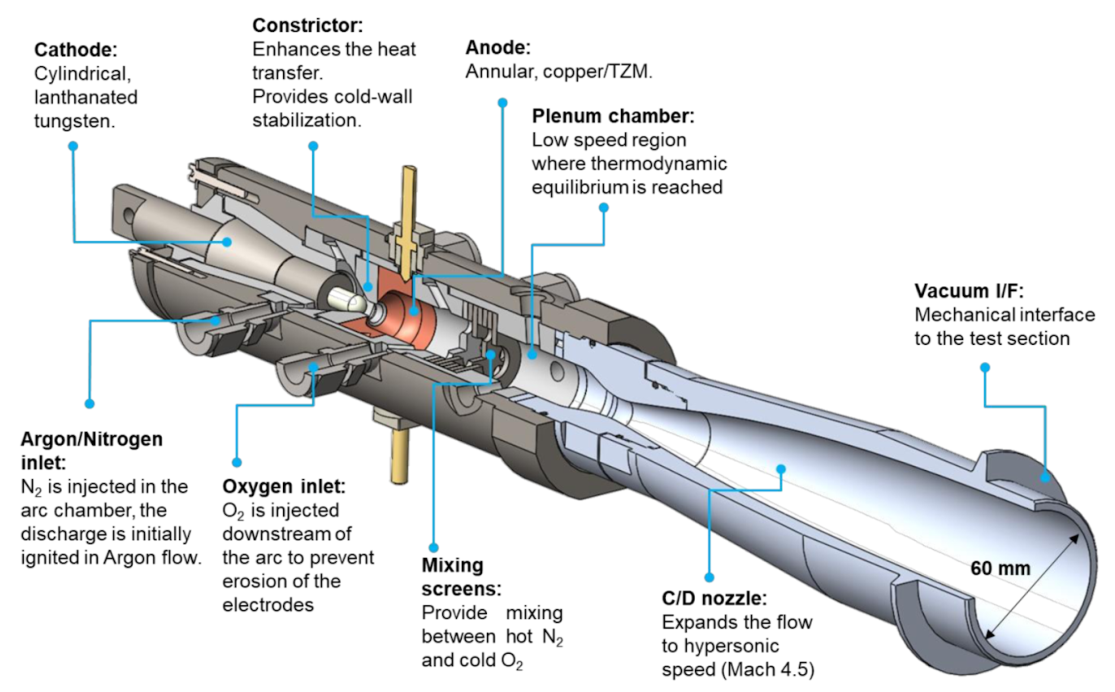
\includegraphics[height=1.75in]{Figures/ACTII.pdf}
%	  		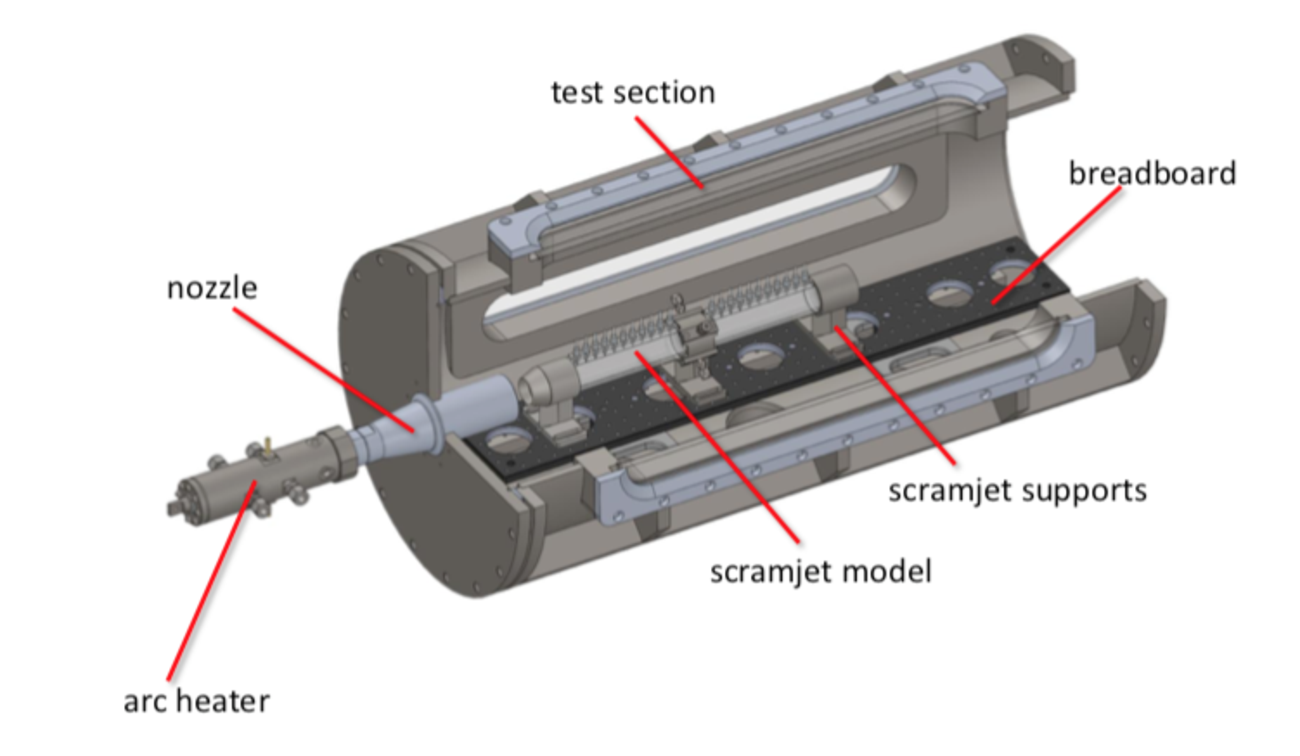
\includegraphics[height=1.6in]{Figures/ACTII_testChamber.pdf}
%	  	\end{figure}
%
%	\end{minipage}
%	\begin{minipage}{0.39\textwidth}
%	\begin{figure}
%		%\vspace{12pt}
%		\centering
%	  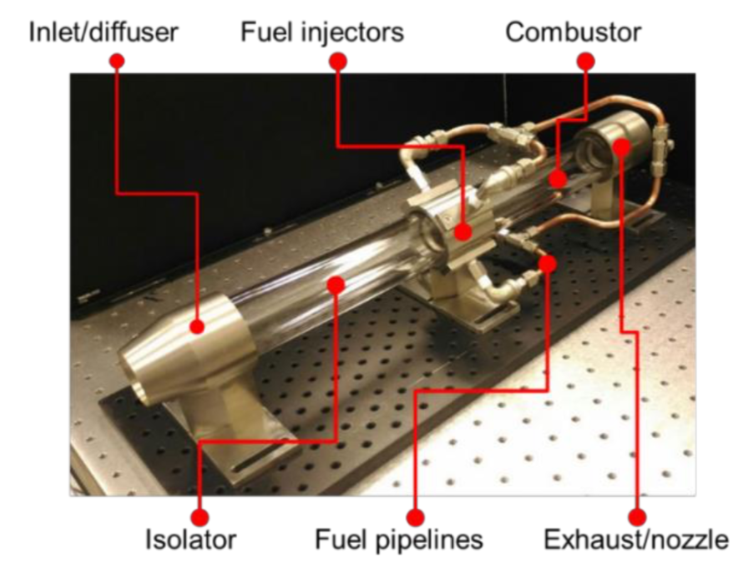
\includegraphics[height=1.4in]{Figures/scramjetModel.pdf}
%	\end{figure}
%	
%		\begin{singlespace} 
%		\tiny Baccarella, Experimental Study of Flow Choking and Inlet Unstart in an Axisymmetric Model Scramjet. 2018. University of Illinois.
%		\end{singlespace}
%	\end{minipage}
%
%
%\end{frame}
%
%\begin{frame}\frametitle{Modeling Timeline Y0/Y1}
%\cPI {Goal:} \PCtwo~simulations provide Y1 prediction and development milestones for \ceesdcode
%
%\hfill
%
%\cPI{Y0 Target:} October 2020
%\begin{itemize}
%	\item Low enthalpy, unstart by mass injection
%	\begin{itemize}
%	\item $CO_2$ flow, $N_2$ injection
%	\item 4 port, supersonic injection
%	\end{itemize}
%\end{itemize}
%
%\cPI{Y1 Target:} Winter 2020/Spring 2021
%\begin{itemize}
%\item High enthalpy, unstart by mass injection
%\begin{itemize}
%\item 16 port injector, air injection
%\end{itemize}
%\item High enthalpy, unstart by combustion
%\begin{itemize}
%\item 16 port injector, $C_2H_4$ injection, auto-ignition
%\end{itemize}
%\end{itemize}
%
%
%\end{frame}
%%======================================================================
%
%\begin{frame}\frametitle{Y1 Prediction Targets}
%
%\begin{minipage}{0.49\textwidth}
%\cPI{Qualitative}
%\begin{itemize}
%\item Unstart Go/No-Go
%\item PLRS comparison
%\end{itemize}
%
%\cPI{Quantitative}
%\begin{itemize}
%\item Scramjet model pressure
%\item Shock/pressure oscillation frequency
%\end{itemize}
%\end{minipage}
%\begin{minipage}{0.49\textwidth}
%\centering
%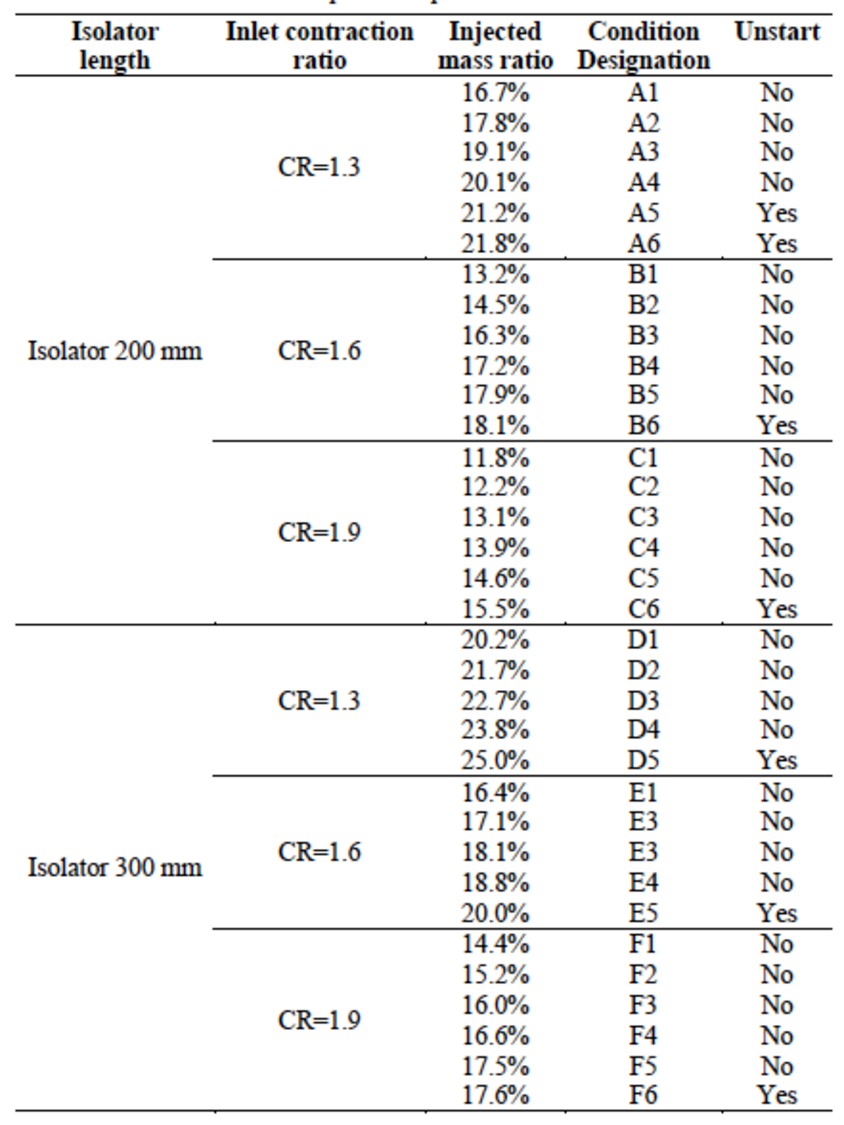
\includegraphics[height=1.7in]{Figures/Go-NoGo.pdf}
%\end{minipage}
%
%\centering
%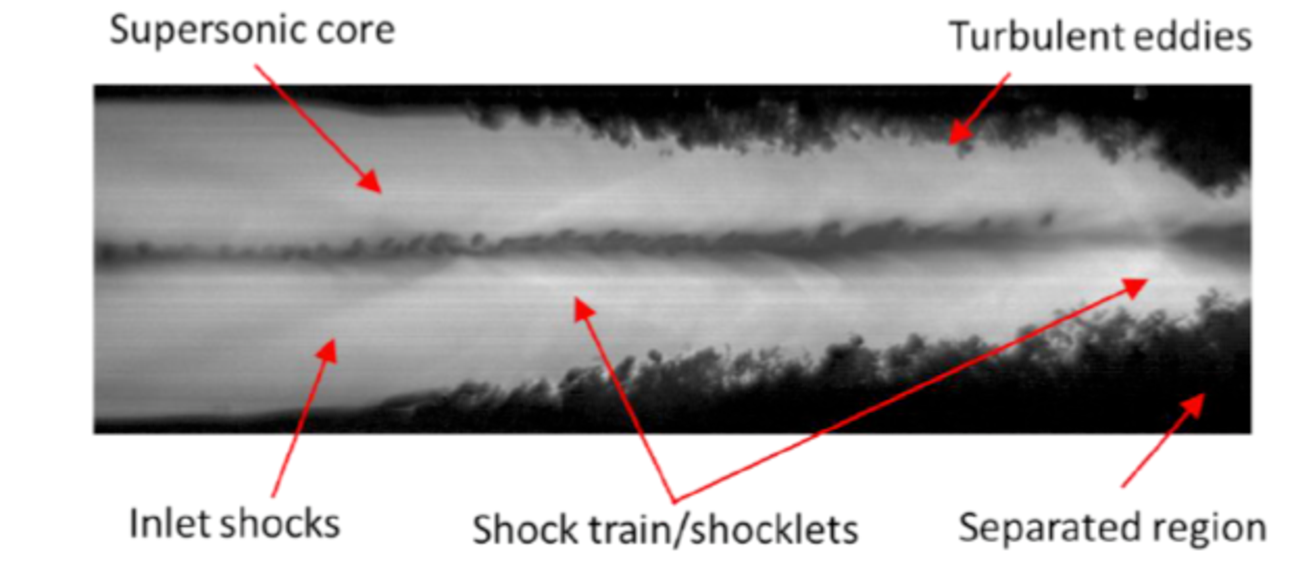
\includegraphics[width=.7\textwidth]{Figures/PLRS-1.pdf}
%
%\end{frame}
%
%
%
%%======================================================================
%
%
%\begin{frame}\frametitle{Numerical Setup - PlasCom2}
%
%\vspace{10pt}
%	\begin{minipage}{0.59\textwidth}
%	  \begin{itemize}
%	    \item Mesh generation tool based on CAD
%	    \item Nine overset meshes
%	    \item Variable resolution in nozzle, scramjet model
% 	    \begin{itemize}
%			\item HalfX - $9.8 M$
%			\item OneX - $69 M$
%			\item OneX+ - $170 M$
%			\item OneX++ - $973 M$
% 	    \end{itemize}
%	    \item OneX resolution sufficient to resolve inlet shocks and nozzle boundary layer
%	    \item Increase scramjet interior resolution to capture turbulence leading to unstart
%	  \end{itemize}
%	\end{minipage}
%	\begin{minipage}{0.39\textwidth}
%	\begin{figure}
%
%		\centering
%	  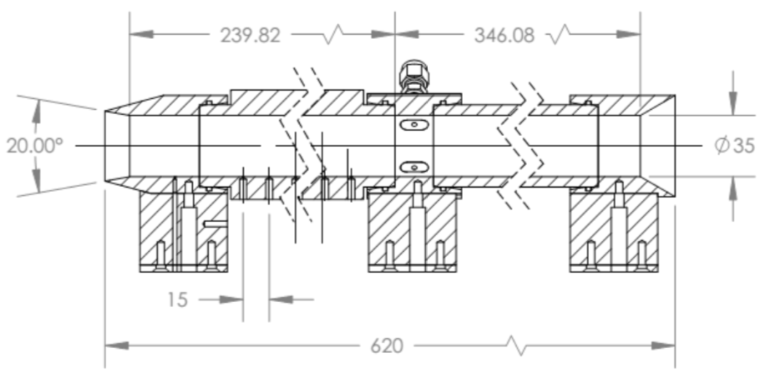
\includegraphics[width=2in]{Figures/CAD.pdf}
%	\end{figure}
%	\vspace{-15pt}
%	\begin{figure}
%		\centering
% 		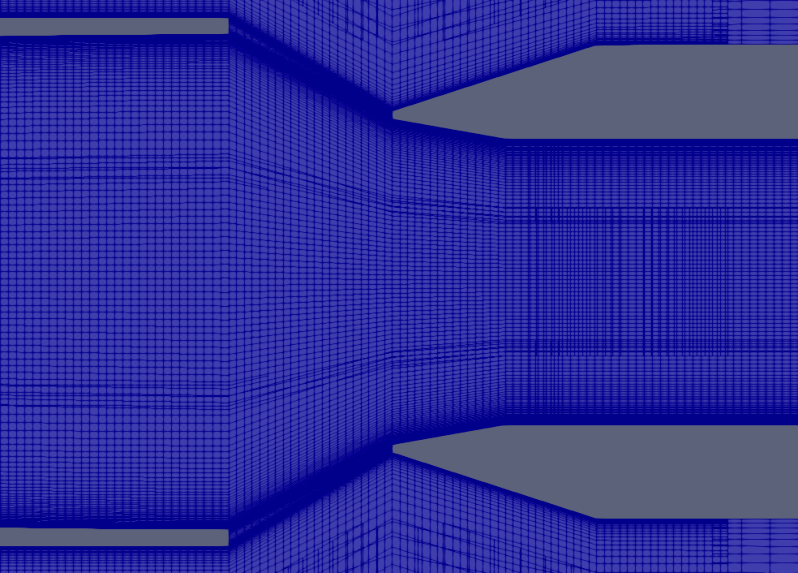
\includegraphics[width=1.4in]{Figures/inletMesh.pdf}
%	\end{figure}
%	\end{minipage}
%	\begin{figure}
%	\centering
%	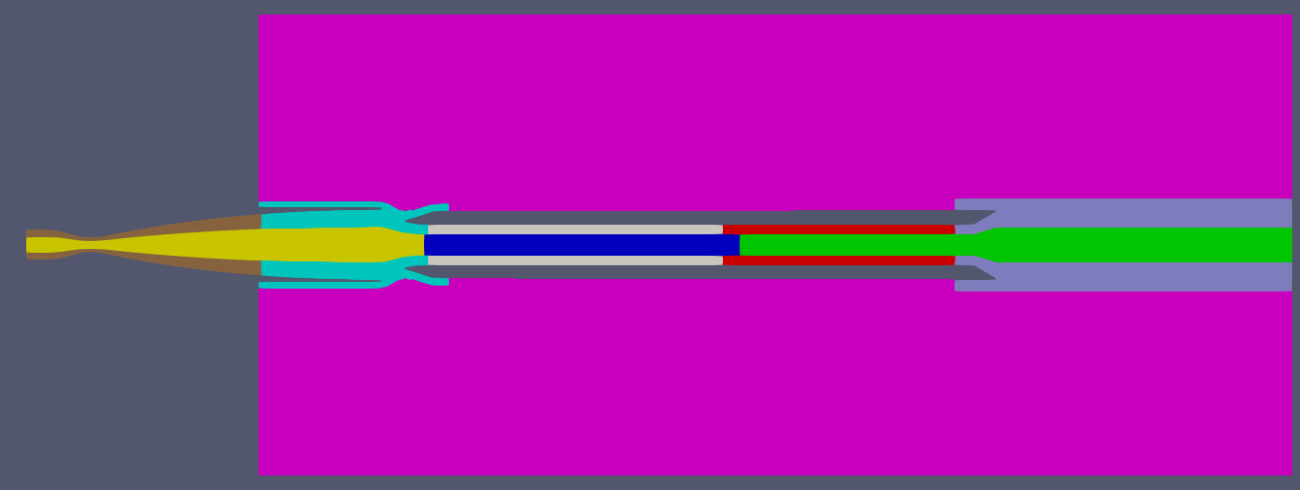
\includegraphics[height=.9in]{Figures/meshPieces.pdf}
%	\end{figure}
%
%\end{frame}
%
%\begin{frame}
%physics (eqns)
%eos (model closure)
%boundary conditions (numerical closure)
%initialization
%sample results
%\end{frame}
%
%%\begin{frame}\frametitle{HalfX vs OneX}
%%
%%  \cPI{Y0 flowthrough}
%%  \begin{itemize}
%%    \item Qualitative comparison, $2.22x10^{-3} s$
%%    \item Constant gamma EOS
%%	\end{itemize}
%%
%%  \begin{figure}
%%  \centering
%%    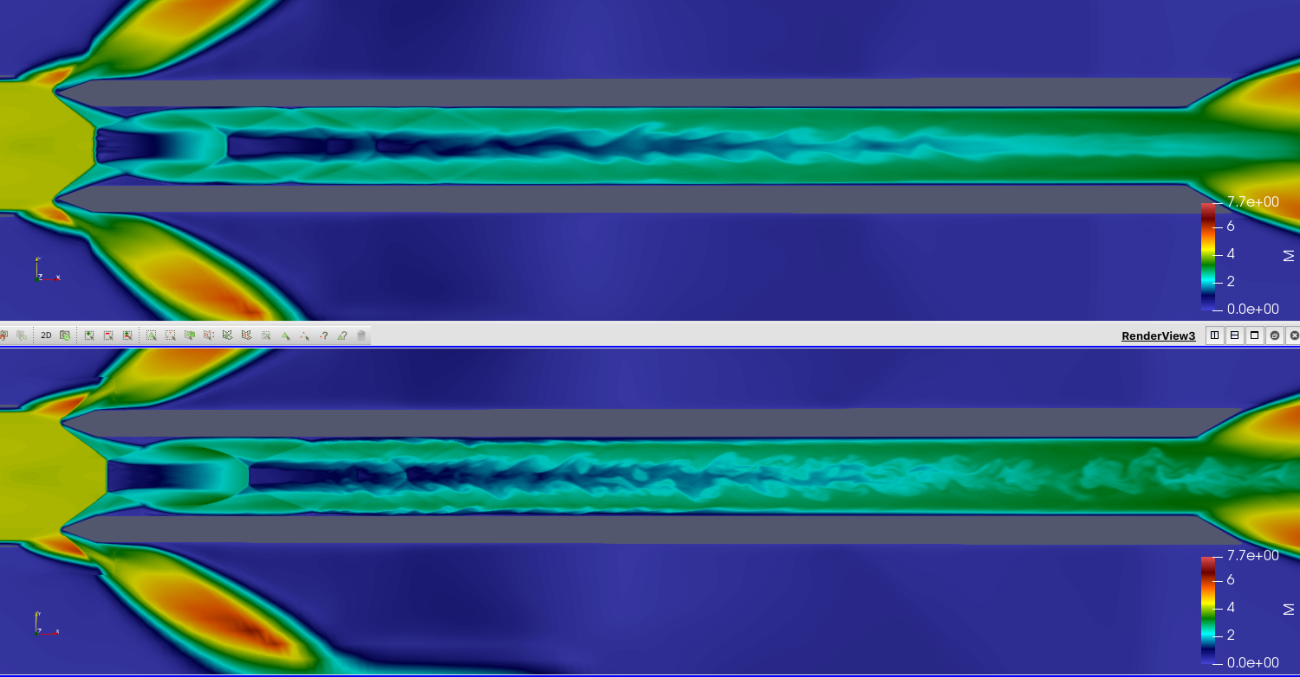
\includegraphics[height=2.in]{figures/halfx_v_onex_M.pdf}
%%  \end{figure}
%%\end{frame}
%
%
%
%\begin{frame}\frametitle{Sample Scramjet Interior Pressure?}
%
%   \vspace{10pt}
%	\begin{figure}
%		%\vspace{12pt}
%		\centering
%	  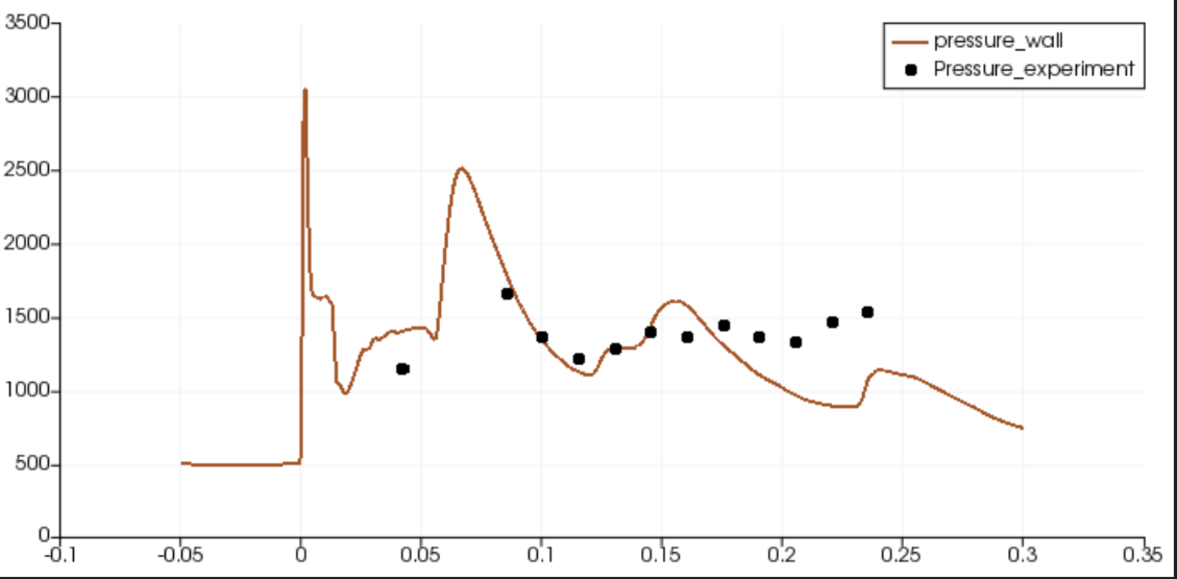
\includegraphics[height=1.4in]{Figures/scramjetPressure.pdf}
%	\end{figure}
%
%	 \begin{itemize}
%	  \item Favorable comparison for initial shock structures
%	  \item Under-resolved BL structures?
%	 \end{itemize}
%	 
%\end{frame}
%	 
%
%       
%	 
%
%
%
%
%
%
%%======================================================================
%\begin{frame}\frametitle{}
%
%\vspace*{0.2in}
%
%\begin{center}
%
%
\includegraphics[width=0.5\textwidth]{Figures/ceesd-logo-2.pdf}
%
%\vspace*{0.35in}
%\cPI{\huge Questions?}
%
%\vspace*{0.5in}
%\begin{minipage}{0.8\textwidth}
%This material is based in part upon work supported by the Department of Energy, National Nuclear Security Administration, under Award Number \textit{TBD}. 
%\end{minipage}
%
%\end{center}
%
%
%\end{frame}
%%======================================================================
%
% 

\end{document}


